%% Springer Nature sn-jnl version of the elliptic-interface paper.
%% Math and Physical Sciences, numbered reference style.
%% Submit as ONE .tex file; attach figures separately.

\documentclass[pdflatex,sn-mathphys-num]{sn-jnl}% Math and Physical Sciences Numbered Reference Style

%%%% Standard Packages
\usepackage{graphicx}%
\usepackage{multirow}%
\usepackage{amsmath,amssymb,amsfonts}%
\usepackage{amsthm}%
\usepackage{mathrsfs}%
\usepackage[title]{appendix}%
\usepackage{xcolor}%
\usepackage{textcomp}%
\usepackage{manyfoot}%
\usepackage{booktabs}%
\usepackage{algorithm}%
\usepackage{algorithmicx}%
\usepackage{algpseudocode}%
\usepackage{listings}%

%% Added for the baseline block diagram.
\usepackage{tikz}
\usetikzlibrary{arrows.meta,positioning,fit,backgrounds}

%% theorem styles (kept from template; available if you later add proofs)
\theoremstyle{thmstyleone}%
\newtheorem{theorem}{Theorem}%
\newtheorem{proposition}[theorem]{Proposition}%
\theoremstyle{thmstyletwo}%
\newtheorem{example}{Example}%
\newtheorem{remark}{Remark}%
\theoremstyle{thmstylethree}%
\newtheorem{definition}{Definition}%

\raggedbottom

\begin{document}

\title[AD-free wavelet operational-matrix method for elliptic interface problems]{An AD-free wavelet operational-matrix method with domain decomposition for elliptic interface problems}

%%=============================================================%%
%% TODO: replace with the real author/affiliation details.     %%
%%=============================================================%%
\author*[1]{\fnm{First} \sur{Author}}\email{iauthor@gmail.com}

\author[1]{\fnm{Second} \sur{Author}}\email{iiauthor@gmail.com}

\affil*[1]{\orgdiv{Department}, \orgname{Organization}, \orgaddress{\street{Street}, \city{City}, \postcode{000000}, \state{State}, \country{Country}}}

%%==================================%%
%% Abstract                          %%
%% Draft below -- replace with your own wording if you prefer.  %%
%% (No citations or equations are allowed in the abstract.)     %%
%%==================================%%
\abstract{Elliptic interface problems carry a solution that is continuous across the interface but whose normal derivative jumps, a kink that a standard physics-informed neural network smears because a single smooth network cannot represent it. We adapt the automatic-differentiation-free wavelet operational-matrix physics-informed neural network to this setting. The solution is written as a fixed sum of Gaussian-derivative wavelets, so every derivative becomes a precomputed constant matrix and the linear problem reduces to a single weighted least-squares solve, with no iterative training. To admit the kink we carry two independent expansions, one per subdomain, coupled only through the interface conditions, so the kink emerges from the coupling rather than from refinement of the basis. Where the geometry is sharp we add finer wavelets only in a band around the interface. On a manufactured benchmark the method holds a relative $L^2$ error between $10^{-3}$ and $10^{-6}$ across contrasts as large as $10^6$, resolves a sharp eight-tooth gear interface through banded refinement, and carries over to the indefinite Helmholtz operator at no real cost. On the gear it beats a tuned least-squares baseline by one to two orders, while iterative networks trained on a fixed budget fail to resolve the toothed interface at all. The forward solve is sub-second, which keeps an outer shape- or contrast-recovery loop cheap; we recover an interface radius from sparse, noisy interior data.}

\keywords{Physics-informed neural networks, Wavelet operational matrix, Elliptic interface problems, Domain decomposition, Least-squares collocation, Inverse problems}

\pacs[MSC Classification]{65N35, 65N21, 68T07, 35J25}

\maketitle

%% ============================================================
\section{Introduction}\label{sec:intro}

Many models in physics and engineering reduce to a second-order elliptic equation in which the material coefficient is not uniform over the domain. When two materials meet along a curve, the coefficient jumps across that curve. We call the curve the \emph{interface} and the resulting model an \emph{elliptic interface problem}. On a bounded domain $\Omega\subset\mathbb{R}^2$ that a closed interface $\Gamma$ splits into an inside region $\Omega^-$ and an outside region $\Omega^+$, the problem reads
\begin{equation}
-\nabla\!\cdot\!\big(a(x)\,\nabla u\big)=f \ \text{ in }\Omega,
\qquad
a(x)=\begin{cases} a^- & x\in\Omega^-,\\[2pt] a^+ & x\in\Omega^+,\end{cases}
\label{eq:intro-pde}
\end{equation}
with $a^-,a^+>0$ constant in each region, a source $f$, and a Dirichlet condition $u=h$ on the outer boundary $\partial\Omega$. The ratio $\rho=a^+/a^-$ is the contrast.

Problems of this form are common. Steady heat conduction between two solids of different conductivity, the electric potential in media of different permittivity, pressure in porous flow through layered soils, and potentials inside and outside a biological cell all take the form of Eq.~\eqref{eq:intro-pde}. In each the coefficient is piecewise constant, and the contrast $\rho$ can be large.

The mathematical feature that sets these problems apart sits at $\Gamma$. The coefficient $a$ is discontinuous there, so Eq.~\eqref{eq:intro-pde} cannot be read pointwise across the interface. The weak form supplies the two conditions that close it,
\begin{equation}
[\![u]\!]=0
\qquad\text{and}\qquad
[\![a\,\partial_n u]\!]=0
\quad\text{on }\Gamma,
\label{eq:intro-jumps}
\end{equation}
where $[\![\cdot]\!]$ denotes the jump across $\Gamma$ and $\partial_n$ the outward-normal derivative: the solution is continuous and the normal flux $a\,\partial_n u$ is continuous. Because $a$ jumps while $a\,\partial_n u$ does not, the normal derivative itself must jump to compensate,
\begin{equation}
\partial_n u^+ \;=\; \frac{a^-}{a^+}\,\partial_n u^- \;=\; \frac{1}{\rho}\,\partial_n u^-.
\label{eq:intro-kink}
\end{equation}
Thus $u$ is continuous but not continuously differentiable: it carries a \emph{kink} across $\Gamma$, $C^0$ but not $C^1$, and that kink sharpens as $\rho$ moves away from one. Reproducing it is the difficulty any solver must face.

Classical solvers handle the kink through the mesh. Finite element methods align the elements with $\Gamma$, and the immersed interface method and its relatives correct the finite-difference stencil near $\Gamma$. These methods are accurate, but they need a mesh that conforms to (or is corrected at) the interface. This is awkward for involved geometries, and the mesh must be rebuilt whenever the interface moves, as it does when the shape itself is the unknown.

Physics-informed neural networks (PINNs) remove the mesh. They represent $u$ by a single smooth multilayer perceptron (MLP) and fit the residual of Eq.~\eqref{eq:intro-pde} through automatic differentiation. A single smooth network, though, is the wrong object for Eq.~\eqref{eq:intro-jumps}. It is $C^\infty$, so it forces $[\![\partial_n u]\!]=0$ by construction, and spectral bias makes it slow to resolve a sharp gradient. The kink is smeared, and the error grows with $\rho$.

We take a different route. We keep the mesh-free setting but drop both the MLP and the automatic differentiation. We use the wavelet-PINN (W-PINN) of \cite{pandey2026}, recalled in Section~\ref{sec:baseline}, in which $u$ is a fixed finite sum of wavelets and only the coefficients are learned. Because the basis is fixed and every operator here is linear, the derivatives become constant operational matrices and the fit becomes a single linear least-squares solve. To admit the kink we carry two such expansions, one per subdomain, coupled only through Eq.~\eqref{eq:intro-jumps}; the kink then emerges from the coupling rather than from any single basis. Where the geometry is sharp, we add finer wavelets only in a band around $\Gamma$, which buys accuracy without inflating the global basis. The mapping is set out in Section~\ref{sec:proposed} and tested in Section~\ref{sec:results}.

Our main contributions are the following.
\begin{itemize}
\item To the best of our knowledge, the first application of the AD-free wavelet operational-matrix W-PINN to elliptic interface problems.
\item A domain-decomposed (two-expansion) formulation in which the flux kink is produced by the interface coupling rather than by basis refinement.
\item An AD-free assembly of value, Laplacian and normal-derivative operational matrices, solved by one weighted least-squares (SVD) pass, sub-second per solve.
\item Accuracy held at high contrast out to $\rho=10^6$, and a banded multiresolution refinement that resolves a sharp gear interface where tuned PIELM and budgeted MLP/XPINN baselines do not.
\item A no-cost extension to the indefinite Helmholtz operator, and an inverse-recovery study that recovers contrast or interface shape from sparse, noisy data.
\end{itemize}

%% ============================================================
\section{The baseline wavelet-PINN}\label{sec:baseline}

We begin from the wavelet-PINN (W-PINN) architecture in its already-published form. Thus this section only recalls the existing pieces; the new mapping is deferred to Section~\ref{sec:proposed}. The aim here is to fix notation and to make the structure of the baseline solver explicit.

A standard physics-informed neural network represents the unknown field $u$ by a multilayer perceptron (MLP) and forms the differential operator through automatic differentiation. The W-PINN replaces this choice. Instead of an MLP, the solution is written as a fixed, finite sum of wavelets,
\begin{equation}
u(x,y) \;=\; \sum_{n=1}^{N_F} c_n\,\Psi_n(x,y) \;+\; b \;=\; W\,c + b,
\label{eq:expansion}
\end{equation}
where $\Psi_n$ are the basis functions, $c=(c_1,\dots,c_{N_F})$ are the trainable coefficients, $b$ is a scalar bias, and $W$ is the matrix of wavelet values sampled at the collocation points. Actually only the coefficients $c$ and the bias $b$ are learned. The basis itself never changes during training.

The basis is the Gaussian-derivative (``Mexican-hat'') wavelet family, taken as a tensor product in two dimensions. We choose it for two reasons. Firstly, it is smooth, so the expansion is well-behaved. Secondly, it admits closed-form derivatives, which is the property the whole architecture depends on. Each member $\Psi_{j,k}$ carries a scale $j=2^{\ell}$ and a translation $k$; summing over a few levels $\ell$ gives the usual multiresolution representation.

The load-bearing idea of the baseline is the \emph{operational matrix}. Because the basis is fixed and every operator of interest is linear, the action of an operator on $u$ is the action of a constant matrix on $c$. Thus, for the value, the Laplacian and the first derivatives, we precompute
\begin{equation}
W = \big[\Psi_n(x_i)\big],\quad
L = \big[\Delta\Psi_n(x_i)\big],\quad
D_x = \big[\partial_x\Psi_n(x_i)\big],\quad
D_y = \big[\partial_y\Psi_n(x_i)\big],
\label{eq:opmats}
\end{equation}
once, before any optimisation. Applying a derivative is then a single matrix-vector product. We observe that no automatic differentiation is required at any iteration, which is the main computational departure from a conventional PINN.

A further consequence is the optimiser. For a PDE that is linear in $u$ with a fixed basis, the W-PINN objective is a convex quadratic in $c$. Thus its global minimum is a (weighted) linear least-squares solution, and gradient descent is, strictly speaking, the wrong tool. The baseline therefore solves the assembled system directly by least squares rather than by Adam. The MLP-plus-Adam path is retained only for parity with nonlinear examples in the source framework.

Figure~\ref{fig:baseline-block} gives the structural overview. The pipeline is feed-forward and has no recurrent training loop for the linear case: collocation points enter, operational matrices are assembled, the linear system is stacked, and a single least-squares solve returns the coefficients.

\begin{figure}[t]
\centering
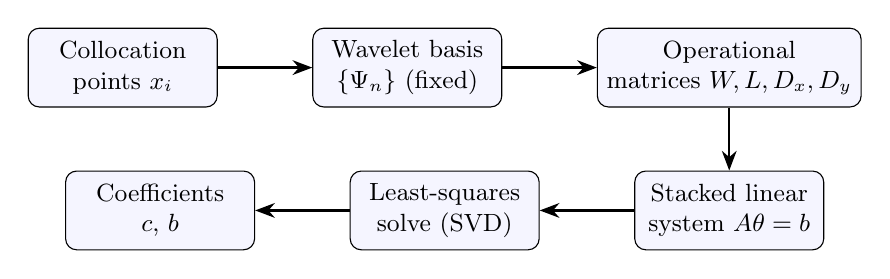
\begin{tikzpicture}[
  node distance=8mm and 12mm,
  box/.style={draw, rounded corners, align=center, minimum height=10mm,
              minimum width=24mm, font=\small, fill=blue!4},
  arrow/.style={-{Stealth[length=2.5mm]}, thick}]
  \node[box] (pts) {Collocation\\points $x_i$};
  \node[box, right=of pts] (basis) {Wavelet basis\\$\{\Psi_n\}$ (fixed)};
  \node[box, right=of basis] (op) {Operational\\matrices $W,L,D_x,D_y$};
  \node[box, below=of op] (sys) {Stacked linear\\system $A\theta=b$};
  \node[box, left=of sys] (solve) {Least-squares\\solve (SVD)};
  \node[box, left=of solve] (out) {Coefficients\\$c,\,b$};
  \draw[arrow] (pts) -- (basis);
  \draw[arrow] (basis) -- (op);
  \draw[arrow] (op) -- (sys);
  \draw[arrow] (sys) -- (solve);
  \draw[arrow] (solve) -- (out);
\end{tikzpicture}
\caption{Structural overview of the baseline W-PINN. The path is feed-forward: the operational matrices are built once, and for a linear PDE a single least-squares solve replaces iterative training.}
\label{fig:baseline-block}
\end{figure}

%% ============================================================
\section{Proposed method: domain-decomposed expansions}\label{sec:proposed}

This section is the core of the paper. We map the baseline of Section~\ref{sec:baseline} onto the elliptic interface problem, and we describe the modifications that this mapping makes necessary. To the best of our knowledge, this is the first application of the AD-free wavelet operational-matrix W-PINN to elliptic interface problems.

\subsection{Target problem}\label{subsec:target}
We solve, on the square $\Omega=(-1,1)^2$,
\begin{equation}
-\nabla\!\cdot\!\big(a(x)\,\nabla u\big) = f \quad\text{in }\Omega,
\qquad
a(x)=\begin{cases} a^- & \text{in } \Omega^-,\\[2pt] a^+ & \text{in } \Omega^+, \end{cases}
\label{eq:pde}
\end{equation}
where a closed interface $\Gamma$ splits $\Omega$ into an inside region $\Omega^-$ and an outside region $\Omega^+$. The coefficient $a$ is piecewise constant, and the ratio $\rho=a^+/a^-$ is the contrast. On the outer boundary we impose a Dirichlet condition $u=h$. On the interface we impose two coupling conditions,
\begin{equation}
[\![u]\!]=0
\qquad\text{and}\qquad
[\![a\,\partial_n u]\!]=0,
\label{eq:jumps}
\end{equation}
i.e. continuity of the solution and continuity of the normal flux, where $[\![\cdot]\!]$ denotes the jump across $\Gamma$ and $\partial_n$ the outward-normal derivative.

The physical subtlety sits in Eq.~\eqref{eq:jumps}. The flux $a\,\partial_n u$ is continuous, yet $a$ jumps. Thus $\partial_n u$ must jump to compensate. The solution is therefore continuous but its gradient is not: $u$ carries a \emph{kink} ($C^0$ but not $C^1$) at the interface. This kink is the feature the method must reproduce.

\subsection{Why one expansion is not enough}\label{subsec:why-two}
A single global expansion of the form~\eqref{eq:expansion} is smooth everywhere it is defined. Thus it forces $[\![\partial_n u]\!]=0$, which violates the flux condition. Instead, we note that the solution is smooth \emph{inside} each subdomain and non-smooth only at the join. We suspect this could be exploited directly, and it can: the kink need not live in any single basis, but can be produced by the coupling of two separate ones.

\subsection{The mapping: domain-decomposed expansions}\label{subsec:mapping}
We therefore carry two independent expansions, one per subdomain,
\begin{equation}
u^- = W^- c^- + b^- \ \text{ in } \Omega^-,
\qquad
u^+ = W^+ c^+ + b^+ \ \text{ in } \Omega^+,
\label{eq:two-exp}
\end{equation}
each of the baseline form~\eqref{eq:expansion}, and we couple them only through the interface conditions~\eqref{eq:jumps}. The unknown vector is $\theta=(c^-,\,c^+,\,b^-,\,b^+)$. We observe that the kink now emerges from the coupling rather than from refinement of the basis. This decomposition is the modification that adapts the baseline to the interface setting.

\subsection{Geometry and collocation}\label{subsec:collocation}
The method is mesh-free, so only scattered points are required. We use four point sets. Firstly, interior points on a $90\times90$ grid, partitioned into $\Omega^-$ and $\Omega^+$ by the sign of the level-set; the PDE residual is enforced here. Secondly, $240$ interface points placed on $\Gamma$, each carrying its outward normal $(n_x,n_y)$; the two interface conditions are enforced here. Thirdly, boundary points on the four edges of the square, which all lie in $\Omega^+$; the Dirichlet condition is enforced here. Lastly, a fine test grid, used only for error reporting. We test a circular interface (radius $r_0=0.5$, radial normal) as the canonical benchmark, and a three-lobed ``flower'' interface to demonstrate non-trivial geometry with varying normals and Newton-found interface points.

\subsection{Operational matrices and the assembled system}\label{subsec:assembly}
On each point set we precompute the baseline matrices of Eq.~\eqref{eq:opmats}. The interface flux uses the normal-derivative matrix $D_n = n_x D_x + n_y D_y$. Because $a$ is constant inside each region, the interior residual reduces to a scaled Laplacian. Stacking all conditions gives a single linear system $A\theta=b$ whose rows are summarised in Table~\ref{tab:rows}.

\begin{table}[t]
\caption{Rows of the assembled linear system for the two-expansion W-PINN. The interface rows couple the two otherwise independent subdomains.}\label{tab:rows}%
\begin{tabular}{@{}ll@{}}
\toprule
Condition & Row of $A\theta=b$ \\
\midrule
PDE residual in $\Omega^-$ & $-a^- L^- c^- = f$ \\
PDE residual in $\Omega^+$ & $-a^+ L^+ c^+ = f$ \\
Continuity on $\Gamma$ & $W^+ c^+ + b^+ - W^- c^- - b^- = 0$ \\
Flux on $\Gamma$ & $a^+ D_n^+ c^+ - a^- D_n^- c^- = 0$ \\
Dirichlet boundary & $W_{\mathrm{bc}} c^+ + b^+ = h$ \\
\botrule
\end{tabular}
\end{table}

\subsection{Solver}\label{subsec:solver}
The PDE is linear and the basis is fixed. Thus the objective is a convex quadratic in $\theta$, and we solve it as a weighted linear least-squares problem by SVD (\texttt{gelsd}). Weights $w_{\mathrm{iface}}$ and $w_{\mathrm{bc}}$ balance the few interface and boundary rows against the many interior rows. The condition number of $A$ can be large because the basis is redundant. However, the SVD truncates the negligible singular values, which acts as a mild regularisation, and the solution lives in the well-conditioned coarse subspace. For robustness we also column-normalise (Jacobi preconditioning) and add a small Tikhonov term. The solve is AD-free, non-iterative, and sub-second.

\subsection{Validation construction}\label{subsec:mms}
For tractability, we further assume a manufactured solution so that the error can be measured exactly. We pick a level-set $\varphi$ (the interface is $\varphi=0$) and set $u=\varphi/a$ per region. For $\varphi=x^2+y^2-r_0^2$ this makes both jump conditions in~\eqref{eq:jumps} hold automatically and gives a constant source $f=-\Delta\varphi=-4$. Thus the exact $u$ is known, and we report the relative $L^2$ error, the maximum error, and an interface-specific flux-kink error.

%% ============================================================
\section{Results}\label{sec:results}

We now report the behaviour of the proposed method. The account runs from a one-dimensional contrast sweep, through the two-dimensional forward problem on three geometries, a refinement-and-conditioning study, a head-to-head against neural and least-squares baselines, robustness at extreme contrast, and a Helmholtz extension, to an inverse-recovery case study at the end.

\subsection{One-dimensional contrast sweep}\label{subsec:1d}
We first isolate the contrast effect in one dimension, where the kink is easiest to inspect. Figure~\ref{fig:phase1} summarises the sweep. We observe that the decomposed wavelet solver stays accurate as $\rho$ grows, with relative $L^2$ error of order $10^{-5}$--$10^{-6}$ and the flux-kink captured essentially exactly. The strongest neural baseline (a decomposed MLP, i.e. an XPINN) behaves differently. Its kink error grows from about $10^{-3}$ at low contrast to roughly $0.12$ at $\rho=10^4$. Thus the advantage of the proposed mapping \emph{widens} with contrast, which is precisely the regime where conventional methods struggle most.

\begin{figure}[t]
\centering

\includegraphics[width=0.9\textwidth]{phase1_summary}
\caption{One-dimensional contrast sweep. The decomposed wavelet solver holds its accuracy across $\rho$, while the MLP/XPINN baseline degrades, most visibly in the flux-kink at high contrast.}
\label{fig:phase1}
\end{figure}

A short ablation supports the claim of Section~\ref{subsec:why-two}. Replacing the two expansions by a single expansion with the \emph{same} basis raises the error by about $360\times$. We suspect this could be due to the single basis being unable to place the kink. The contrast comparison against the MLP baseline is collected in Table~\ref{tab:contrast}.

\begin{table}[t]
\caption{Contrast sweep, representative orders of magnitude. The wavelet solver is AD-free and sub-second per solve; the baseline is trained with Adam. The gap grows with $\rho$.}\label{tab:contrast}%
\begin{tabular}{@{}rcccc@{}}
\toprule
$\rho$ & wavelet rel.\ $L^2$ & wavelet kink err. & XPINN rel.\ $L^2$ & XPINN kink err. \\
\midrule
$10$    & $\sim10^{-6}$ & $\sim10^{-6}$ & $\sim10^{-3}$ & $\sim10^{-3}$ \\
$10^2$  & $\sim10^{-6}$ & $\sim10^{-6}$ & $\sim10^{-3}$ & $\sim10^{-2}$ \\
$10^3$  & $\sim10^{-5}$ & $\sim10^{-5}$ & $\sim10^{-2}$ & $\sim10^{-2}$ \\
$10^4$  & $\sim10^{-5}$ & $\sim10^{-5}$ & $\sim10^{-1}$ & $\sim0.12$ \\
\botrule
\end{tabular}
\end{table}

\subsection{Two-dimensional forward problem}\label{subsec:2d}
We next move to two dimensions. Figure~\ref{fig:circle} shows the circular interface at $\rho=1000$: the exact field, the wavelet prediction, the pointwise error map, and a radial slice along $y=0$. We observe that the slice reproduces the kinks at $\pm r_0$, and the error map stays below the $10^{-6}$ level over most of the domain. Thus the qualitative kink behaviour and the quantitative accuracy agree.

\begin{figure}[t]
\centering

\includegraphics[width=0.95\textwidth]{sol}
\caption{Circular interface ($\rho=1000$). From left to right: exact solution, wavelet W-PINN prediction, $\log_{10}$ error, and the slice $y=0$ showing the gradient kinks at $\pm r_0$.}
\label{fig:circle}
\end{figure}

Figure~\ref{fig:flower} repeats the experiment on the flower interface. The geometry here is non-trivial: the normal varies along $\Gamma$, and the interface points are found by a Newton step. We observe that the accuracy is preserved, which indicates that the mapping is not tied to the radial symmetry of the circle.

\begin{figure}[t]
\centering

\includegraphics[width=0.95\textwidth]{sol1}
\caption{Flower interface. The varying normal and the irregular shape are handled without remeshing, and the kink along $\Gamma$ is preserved.}
\label{fig:flower}
\end{figure}

On the conditioning side, we note a trade-off rather than a free lunch. Adding wavelet levels improves accuracy by roughly an order of magnitude per level, but it also raises the condition number. For tractability, we further assume a parsimonious basis of three levels $[0,1,2]$. This sits near the sweet spot: in one dimension a ten-level basis reaches a condition number of order $10^{196}$, whereas the three-level basis in two dimensions stays near $10^{21}$, which the SVD handles cleanly.

\subsection{Banded refinement: the gear interface}\label{subsec:gear}
The circle and the flower are smooth. We finally test a geometry with sharp features: an eight-tooth gear interface ($N=8$ teeth, base radius $R_0=0.55$, tooth amplitude $B=0.04$, sharpness $s=8$), whose tooth tips reach about $44\%$ of the base radius in radial depth. The tips are near-cusps, so the kink there is harder to place than on the smooth shapes. A uniformly fine basis would resolve them, but at a cost: the finest level over the whole square is about $9600$ functions, which is impractical for the dense least-squares solve.

We instead refine only where the geometry asks for it. The coarse levels $[0,1,2,3]$ are kept global, and the two finest levels $[4,5]$ are placed only in the annular band $r\in(0.42,0.86)$ that holds the teeth. This banded basis has $N_F=4764$ functions, against the $\sim9600$ of a global finest level. Because the kink is local to $\Gamma$, the fine wavelets are spent only where they act. Figure~\ref{fig:gear} shows the result at $\rho=10$.

\begin{figure}[t]
\centering

\includegraphics[width=0.95\textwidth]{sol12}
\caption{Gear interface ($\rho=10$, eight teeth). From left to right: exact solution, wavelet W-PINN prediction, and the $\log_{10}$ error map (panel c). The residual concentrates at the sharp tooth tips, while the bulk of the domain stays near $10^{-4}$.}
\label{fig:gear}
\end{figure}

Table~\ref{tab:gear-contrast} reports the gear across contrast. The relative $L^2$ error stays near $10^{-3}$ across two orders of magnitude in $\rho$, and the bulk error sits near $10^{-4}$. We observe that the worst-case $L^\infty$ and the flux-kink errors are localised at the tooth tips, as panel~(c) of Figure~\ref{fig:gear} shows; away from the tips the field is recovered to the bulk level.

\begin{table}[t]
\caption{Gear interface across contrast (banded basis, $N_F=4764$). The relative $L^2$ error holds near $10^{-3}$, and the worst-case errors stay confined to the sharp tooth tips.}\label{tab:gear-contrast}%
\begin{tabular}{@{}rccc@{}}
\toprule
$\rho$ & rel.\ $L^2$ & $L^\infty$ & kink err. \\
\midrule
$10$    & $1.68\times10^{-3}$ & $1.15\times10^{-3}$ & $1.00\times10^{-2}$ \\
$100$   & $4.98\times10^{-4}$ & $5.63\times10^{-4}$ & $1.21\times10^{-2}$ \\
$1000$  & $1.02\times10^{-3}$ & $5.06\times10^{-4}$ & $2.11\times10^{-2}$ \\
\botrule
\end{tabular}
\end{table}

The banded refinement is what carries the sharp geometry. Table~\ref{tab:gear-band} isolates its effect at $\rho=10$. Adding the two finest levels in the teeth band alone lowers the relative $L^2$ error by about $13\times$ and the worst-case $L^\infty$ by about $10\times$, at the price of a few hundred extra basis functions, far cheaper than a global finest level. Thus the multiresolution structure of the basis does work that a fixed-coordinate single-resolution network cannot: the refinement is steered to the interface without remeshing.

\begin{table}[t]
\caption{Banded refinement against a global coarse basis on the gear interface ($\rho=10$). Placing the finest wavelets only in the teeth band improves the relative $L^2$ error by roughly $13\times$ for a few hundred extra functions.}\label{tab:gear-band}%
\begin{tabular}{@{}lrccc@{}}
\toprule
Basis & $N_F$ & rel.\ $L^2$ & $L^\infty$ & kink err. \\
\midrule
$[0,1,2,3]$ global & $2500$ & $2.25\times10^{-2}$ & $1.14\times10^{-2}$ & $6.89\times10^{-2}$ \\
$[0,1,2,3]+$band$[4,5]$ & $4764$ & $1.68\times10^{-3}$ & $1.15\times10^{-3}$ & $1.00\times10^{-2}$ \\
\botrule
\end{tabular}
\end{table}

\subsection{Refinement and conditioning}\label{subsec:conv}
How far should the banded refinement go? We push it one level at a time on the gear at $\rho=10$ and watch the error and the conditioning together. Table~\ref{tab:conv} collects the sweep and Figure~\ref{fig:conv} plots it. The first two steps behave as hoped. The global coarse basis sits at $2.25\times10^{-2}$; adding band $[4]$ drops it to $3.4\times10^{-3}$; band $[4,5]$ reaches $1.7\times10^{-3}$. The fourth step breaks the trend. Band $[4,5,6]$ pushes $N_F$ past twelve thousand, drives the condition number beyond $10^{32}$, and the relative error climbs back to $3.4\times10^{-1}$, worse than the coarse basis it started from.

What we are looking at is a valley, not a slope. Accuracy falls while the new wavelets still carry signal, then reverses once the design matrix grows too ill-conditioned for the SVD to separate the useful directions from the noise. The banded $[4,5]$ basis sits at the bottom, and that is why we keep it throughout the paper. We read the upturn not as a failure of multiresolution refinement as such, but as the point where a redundant, fixed basis stops paying its way.

\begin{table}[t]
\caption{Refinement sweep on the gear ($\rho=10$). Error falls through band $[4,5]$, then the condition number overwhelms the SVD and accuracy reverses. The parsimonious $[4,5]$ basis is the adopted choice.}\label{tab:conv}%
\begin{tabular}{@{}lrcccc@{}}
\toprule
Basis & $N_F$ & rel.\ $L^2$ & $L^\infty$ & kink err. & cond.\ no. \\
\midrule
$[0,1,2,3]$ global & $2500$  & $2.25\times10^{-2}$ & $1.16\times10^{-2}$ & $6.89\times10^{-2}$ & $3.4\times10^{19}$ \\
$+\,$band$[4]$     & $2948$  & $3.37\times10^{-3}$ & $4.34\times10^{-3}$ & $2.23\times10^{-3}$ & $5.5\times10^{18}$ \\
$+\,$band$[4,5]$   & $4764$  & $1.68\times10^{-3}$ & $1.15\times10^{-3}$ & $1.00\times10^{-2}$ & $4.8\times10^{20}$ \\
$+\,$band$[4,5,6]$ & $12028$ & $3.44\times10^{-1}$ & $1.42\times10^{-1}$ & $9.74\times10^{0}$  & $2.8\times10^{32}$ \\
\botrule
\end{tabular}
\end{table}

\begin{figure}[t]
\centering

\includegraphics[width=0.8\textwidth]{convergence}
\caption{Refinement on the gear ($\rho=10$): relative $L^2$ error and condition number against the added wavelet level. The error reaches its minimum at the banded $[4,5]$ basis and rises again once the conditioning degrades.}
\label{fig:conv}
\end{figure}

\subsection{Head-to-head with neural and least-squares baselines}\label{subsec:baselines}
We place the method against the solvers a reader would reach for, all on the same gear, with the radial-basis solver given the same basis size as ours ($N_F=4764$). Table~\ref{tab:baselines} reports two contrasts.

The physics-informed extreme learning machine (PIELM) with radial-basis features is the nearest relative: like ours it fits a single least-squares system and trains nothing iteratively. It is also the most temperamental of the group. Its accuracy hangs on the shape parameter $\varepsilon$; at $\rho=10$ the best value we found ($\varepsilon=5$) returns $9.0\times10^{-2}$, while the settings on either side scatter from $1.2\times10^{-1}$ up past unity. The wavelet basis has no such dial, and at the same contrast it gives $1.7\times10^{-3}$, between one and two orders below even the best-tuned PIELM. At $\rho=1000$ the ordering is unchanged.

The trained networks do worse on this geometry. Inside a fixed budget of eight thousand Adam iterations, neither the decomposed MLP (XPINN) nor a single MLP brought the relative error under one; on a toothed interface, in the time allowed, both effectively failed to resolve the field. We give the numbers for completeness and state the caveat plainly: these are budgeted runs, not converged ones, and a longer schedule would improve them. The least-squares solvers need no such schedule, and once the operational matrices are built the solve itself is sub-second.

\begin{table}[t]
\caption{Head-to-head on the gear, relative $L^2$ and $L^\infty$ error. The radial-basis PIELM is matched to the wavelet basis size ($N_F=4764$); the MLPs are trained for $8\times10^3$ Adam iterations (a fixed budget, not convergence).}\label{tab:baselines}%
\begin{tabular*}{\textwidth}{@{\extracolsep\fill}lcccc@{}}
\toprule
& \multicolumn{2}{@{}c@{}}{$\rho=10$} & \multicolumn{2}{@{}c@{}}{$\rho=1000$} \\\cmidrule{2-3}\cmidrule{4-5}
Method & rel.\ $L^2$ & $L^\infty$ & rel.\ $L^2$ & $L^\infty$ \\
\midrule
Wavelet W-PINN (banded)   & $1.68\times10^{-3}$ & $1.15\times10^{-3}$ & $1.02\times10^{-3}$ & $5.06\times10^{-4}$ \\
RBF-PIELM ($\varepsilon=5$, best) & $8.97\times10^{-2}$ & $3.33\times10^{-2}$ & $1.61\times10^{-2}$ & $7.03\times10^{-3}$ \\
RBF-PIELM ($\varepsilon=12$) & $1.40\times10^{-1}$ & $5.12\times10^{-2}$ & $1.10\times10^{-2}$ & $1.10\times10^{-2}$ \\
XPINN-MLP (Adam $8\mathrm{k}$) & $2.65\times10^{0}$ & $7.91\times10^{-1}$ & $1.97\times10^{0}$ & $5.86\times10^{-1}$ \\
Vanilla MLP (Adam $8\mathrm{k}$) & $4.46\times10^{0}$ & $1.10\times10^{0}$ & $1.01\times10^{0}$ & $3.04\times10^{-1}$ \\
\botrule
\end{tabular*}
\end{table}

\subsection{Robustness at extreme contrast}\label{subsec:extreme}
The two-order range of Table~\ref{tab:gear-contrast} can be stretched in both directions. Table~\ref{tab:extreme} carries the gear out to $\rho=10^6$ and down to $\rho=10^{-3}$. On the high side the solver barely moves: from $\rho=10^4$ to $\rho=10^6$ the relative $L^2$ error stays near $1.1\times10^{-3}$ and the maximum error holds. A contrast of a million is where the flux balance usually slips, so the flatness here is worth recording.

The low side is not the mirror image. At $\rho=10^{-3}$, with the inside stiffer than the outside, the relative $L^2$ error remains small ($2.8\times10^{-4}$), yet the kink error rises to order one and the maximum error to $0.24$. The jump in the normal derivative reverses sign in this regime and piles up at the tooth tips, where the banded basis is already stretched; the bulk field comes back but the tip flux does not. We keep the case in the table rather than drop it. The method is aimed at the high-contrast end, and this asymmetry marks the boundary of where we would trust it.

\begin{table}[t]
\caption{Gear at extreme contrast (banded basis). High contrast is stable to $\rho=10^6$; the $\rho<1$ case keeps a small $L^2$ error but loses the tip flux, where the kink error grows to order one.}\label{tab:extreme}%
\begin{tabular}{@{}rccc@{}}
\toprule
$\rho$ & rel.\ $L^2$ & $L^\infty$ & kink err. \\
\midrule
$10^{-3}$ & $2.79\times10^{-4}$ & $2.44\times10^{-1}$ & $2.34\times10^{0}$ \\
$10^{4}$  & $1.25\times10^{-3}$ & $1.52\times10^{-3}$ & $8.49\times10^{-2}$ \\
$10^{5}$  & $1.09\times10^{-3}$ & $1.69\times10^{-3}$ & $9.50\times10^{-2}$ \\
$10^{6}$  & $1.08\times10^{-3}$ & $1.69\times10^{-3}$ & $9.51\times10^{-2}$ \\
\botrule
\end{tabular}
\end{table}

\subsection{An indefinite operator: the Helmholtz term}\label{subsec:helmholtz}
None of the assembly is bound to the Laplace operator. A reaction term turns Eq.~\eqref{eq:pde} into the interface Helmholtz problem $-\nabla\!\cdot\!(a\nabla u)-k^2 u = f$, still linear in $u$ and indefinite once $k$ is large. In operational-matrix form the change is one block: the interior row picks up a $-k^2 W$ term, and everything else, including the AD-free assembly, is left alone. Table~\ref{tab:helmholtz} runs the gear at wavenumbers $k\in\{2,4,8\}$ for two contrasts. Every entry stays in the $10^{-3}$ band, with none of the breakdown that indefiniteness can produce; the worst of them, $3.5\times10^{-3}$ at $k=4,\ \rho=10$, still falls inside the range of the elliptic runs. The extension costs almost nothing, which is the dividend of keeping the operator linear and the basis fixed.

\begin{table}[t]
\caption{Helmholtz gear, $-\nabla\!\cdot\!(a\nabla u)-k^2u=f$, solved by the same banded wavelet basis and AD-free assembly. Accuracy holds in the $10^{-3}$ band across wavenumbers and contrasts.}\label{tab:helmholtz}%
\begin{tabular}{@{}rrccc@{}}
\toprule
$k$ & $\rho$ & rel.\ $L^2$ & $L^\infty$ & kink err. \\
\midrule
$2$ & $10$   & $1.69\times10^{-3}$ & $1.15\times10^{-3}$ & $9.96\times10^{-3}$ \\
$2$ & $1000$ & $1.03\times10^{-3}$ & $5.04\times10^{-4}$ & $2.10\times10^{-2}$ \\
$4$ & $10$   & $3.53\times10^{-3}$ & $1.15\times10^{-3}$ & $1.21\times10^{-2}$ \\
$4$ & $1000$ & $1.50\times10^{-3}$ & $4.95\times10^{-4}$ & $2.07\times10^{-2}$ \\
$8$ & $10$   & $2.34\times10^{-3}$ & $1.15\times10^{-3}$ & $1.05\times10^{-2}$ \\
$8$ & $1000$ & $9.68\times10^{-4}$ & $4.88\times10^{-4}$ & $2.06\times10^{-2}$ \\
\botrule
\end{tabular}
\end{table}

\subsection{Inverse case study}\label{subsec:inverse}
Finally, we exercise the method on an inverse problem, which is where the sub-second forward solve becomes decisive. Given sparse, noisy interior measurements of $u$, we recover an unknown parameter, namely the contrast or the interface shape. The scheme is an outer loop over the few physical parameters times an inner AD-free forward solve of about $0.4$\,s each; a derivative-free optimiser minimises the interior data misfit. Figure~\ref{fig:inverse} shows the recovery.

\begin{figure}[t]
\centering

\includegraphics[width=0.9\textwidth]{sol2}
\caption{Inverse recovery from sparse interior data. The forward solve is fast enough that an outer optimisation over the unknown parameter remains cheap.}
\label{fig:inverse}
\end{figure}

The recovery is graceful under noise. We observe that even ten interior points at $5\%$ noise recover the radius to about $0.9\%$, and $1\%$ noise gives an error of order $10^{-3}$. We also checked that the result is not an inverse crime. The data is the analytic solution, so the data-generating model differs from the inversion model, and the recovery error tracks the forward discretisation floor ($\sim10^{-6}$) rather than machine precision. When we instead invert an ellipse truth with a wrong (circle) model family, the data residual cannot fall below about $6\times10^{-3}$. Thus a mis-specified model is diagnosable from the residual, which is the opposite of an artifact.

%% ============================================================
\section{Discussion}\label{sec:discussion}

We collect what the experiments imply. The advantage of the method over the neural baselines is not uniform; it concentrates in two regimes. The first is high contrast, where a single smooth network smears the kink and the decomposed wavelet solver does not. The second is sharp geometry, where the multiresolution basis refines only at the interface and a fixed-coordinate network cannot. On the gear the comparison of Section~\ref{subsec:baselines} is one-sided: the best-tuned PIELM trails by one to two orders, and its accuracy swings with a shape parameter that ours does not carry. We still avoid a universal claim. On smooth, low-contrast problems a well-chosen PIELM is a capable solver and our margin narrows; what the experiments show is that the margin widens precisely where the problem is hard.

The accuracy we report, near $10^{-3}$ in two dimensions, is modest against a conforming finite element or immersed interface solver, which reach much smaller errors on the same problem. The trade we offer is different. The solve is mesh-free and AD-free, the forward pass is sub-second, and the interface geometry is a few parameters rather than a mesh. This is what keeps the inverse problem cheap, and it is the setting in which the method earns its place. We read the gear result in the same way: it is a demonstration that refinement can be steered to a sharp interface without remeshing, not a claim of high precision at the tooth tips, where the error stays near $10^{-2}$.

%% ============================================================
\section{Conclusion}\label{sec:conclusion}

We mapped the AD-free wavelet operational-matrix W-PINN onto the elliptic interface problem. The two-expansion decomposition produces the flux kink from the interface coupling, the operational matrices remove automatic differentiation, and the linear problem is one least-squares solve. The method holds its accuracy as the contrast grows, out to a ratio of $10^6$; it handles non-trivial and sharp interface geometry through banded refinement; it carries over to the indefinite Helmholtz operator at no real cost; it outperforms tuned PIELM and budgeted MLP baselines on the toothed interface; and it supports a sub-second inverse recovery from sparse, noisy data.

The studies also draw the boundary of the method. Refinement helps only up to the banded $[4,5]$ basis, beyond which conditioning takes over (Section~\ref{subsec:conv}); and the low-contrast regime $\rho<1$, where the tip flux is under-resolved, is where reliability ends (Section~\ref{subsec:extreme}). These mark the natural next steps: a better-placed basis for the $\rho<1$ flux, multiple disconnected inclusions and re-entrant corners to test the decomposition past a single closed interface, and a convergence theory that would put the valley of Section~\ref{subsec:conv} on firm ground. We expect these to sharpen the trade-off identified here rather than overturn it.

\backmatter

\bmhead{Acknowledgements}
Not applicable.

\section*{Declarations}

\begin{itemize}
\item \textbf{Funding.} Not applicable.
\item \textbf{Conflict of interest.} The authors declare no competing interests.
\item \textbf{Data availability.} The data that support the findings of this study are available from the corresponding author on reasonable request.
\item \textbf{Code availability.} Code available from the corresponding author on reasonable request.
\item \textbf{Author contribution.} TODO.
\end{itemize}

%%===========================================================================%%
%% References. Numbered (sn-mathphys-num). Add the remaining citations        %%
%% (FEM, IIM, PINN, XPINN, PIELM) when ready; only the baseline is listed.    %%
%%===========================================================================%%
\begin{thebibliography}{9}

\bibitem{pandey2026}
Pandey, H., Singh, A., Behera, R.:
An efficient wavelet-based physics-informed neural network for multiscale problems.
Neural Networks \textbf{200}, 108860 (2026)

\end{thebibliography}

\end{document}
